\subsection{Проектирование и разработка серверной части программного средства}
\label{sec:design:server}

Все программное средство разбито на отдельные модули. Это
необходимо для обеспечения гибкой структуры ПО. При данном подходе
допускается модернизация любого из выбранных модулей без изменения
остальных. Появляется возможность адаптировать данное программное
средство для различных платформ.

На каждый логически выделенный блок программы были возлагаются
определенные задачи. Кроме того, каждый блок так или иначе связан с
другими остальными блоками, чтобы обеспечить работоспособность всего
программного средства в целом.

На основе указанных требований продукта можно выделить модули, отвечающими за следующие функции:

\begin{itemize}
	\item работа с данными через протокол HTTPS;
	\item обработка команд;
	\item взаимодействие с базой данных.
\end{itemize}

Структурная схема, иллюстрирующая перечисленные модули и связи
между ними приведена на рисунке \ref{fig:design:architecture:structure_api}. Кроме функциональных модулей на
схеме представлены модуль базы данных и отправки сообщений клиенту.
Каждый из перечисленных модулей системы решает определенные задачи.

\begin{figure}[!h]
\centering
	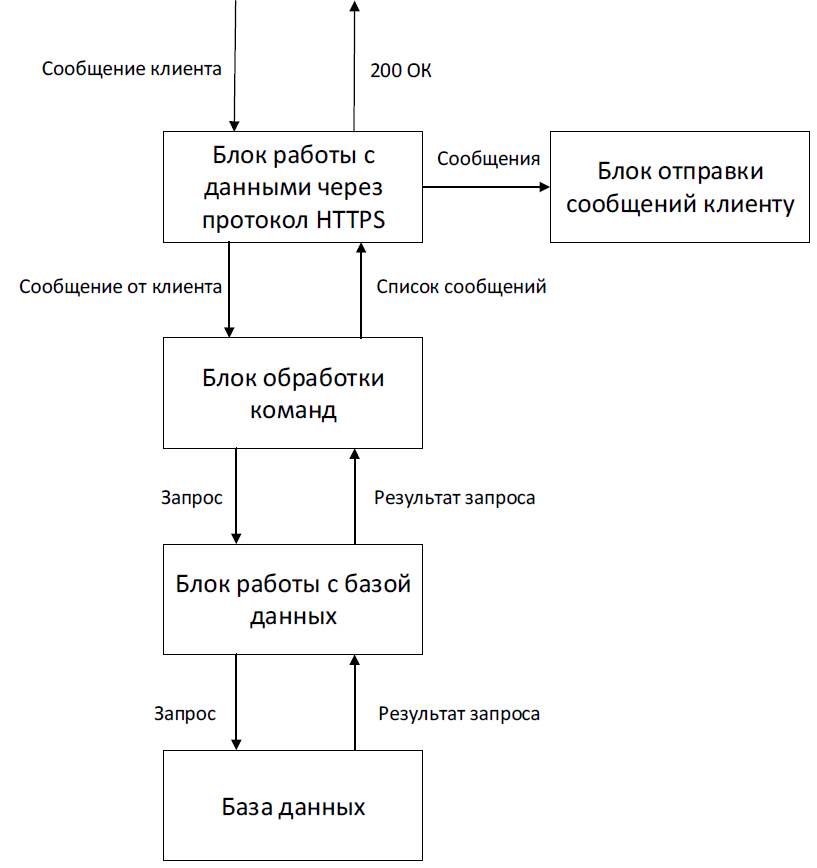
\includegraphics[scale=0.7]{structure_api.png}
	\caption{Схема взаимодействия модулей программного средства}
	\label{fig:design:architecture:structure_api}
\end{figure}
\subsubsection{} Модуль работы с данными через протокол HTTPS
\label{sec:design:server:api}

Отвечает за предоставление данных в определенном формате для клиентских приложений. Реализован в виде сервиса, основанного на \linebreak webhook. Webhooks позволяют уведомить сервера Telegram, что в случае, если появится сообщение для бота, отправлять данное сообщение следует по ссылке, указанной в настройках конфигурации. Отпадает необходимость периодически опрашивать серверы самому, тем самым, снижается риск возникновения исключительных ситуаций в приложении. Однако, за это приходится платить установкой полноценного веб-сервера на машину, где предполагается запуск бота. Также, необходимо иметь SSL сертификат, так как webhooks в Telegram работают только по протоколу HTTPS \cite{web_protocols}.

Модуль содержит в себе единственный контроллер с одним методом GetMessage.

Метод принимает структуру Update, которая содержит в себе все данные о сообщении, в том числе:

\begin{itemize}
	\item Message.Text – текст сообщения;
	\item Message.From.FirstName – имя пользователя;
	\item MessageFrom.LastName – фамилия пользователя;
	\item MessageFrom.ChatId – уникальный идентификатор чата.
\end{itemize}

В случае, если структура содержит в себе не сообщение, а, например, результат нажатия на кнопку InlineButton, то свойство Message будет иметь значение null, а данные будут содержаться в свойстве CallbackQuery.
Если структура не содержит ни текстового сообщения, ни результата нажатия на кнопку, сервером сразу же прерывается выполнение и отправляется ответ с кодом 200.

Основные методы перечислены в таблице \ref{table:design:server:api}.

\begin{longtable}{|>{\raggedright}p{0.3\textwidth}|
		 >{\raggedright}p{0.3\textwidth}|
		 >{\raggedright\arraybackslash}p{0.32\textwidth}|} 
	\caption{Классы и методы модуля работы через протокол HTTPS}
	\label{table:design:server:api}\\

	\hline
	\centering Класс & \centering Метод & \centering\arraybackslash Описание \endfirsthead

	\caption*{Продолжение таблицы \ref{table:design:server:api}}\\\hline
	\centering 1 & \centering 2 & \centering\arraybackslash 3 \\\hline \endhead

	\hline
	\centering 1 & \centering 2 & \centering\arraybackslash 3 \\
	\hline

	FinanceManager
BotController & GetMessage(Update update) & Получает структуру Update, извлекает из нее нужные данные, передает управление в модуль обработки команд. После получения списка сообщений, передает управление в модуль обработки сообщений. \\

	ControllerHelper & BuildKeyBoardMarkup(
List<string> options) & Строит и возвращает структуру InlineKeyBoardMarkup.
В качестве параметра принимает список строк, со значениями которых требуется построить виртуальные кнопки. В случае нечетного количества строк, последняя кнопка будет расположена на всю длину пространства.  \\ 

	& & Вызывается в случае, если для вопроса бота требуется виртуальные кнопки. \\ \hline

	BotExtensions & AddTelegramBot(this IServiceCollection services, IConfigurationRoot configuration) & Добавляет в контейнер Dependency Injection класс-обертку для посылки сообщений. \\ \hline

	BotExtensions & UseTelegramBot(this IApplicationBuilder app, string webhookPath) & Метод расширения IApplicationBuilder. Устанавливает боту адрес webhook. Запускает бот. \\ \hline

	Dependency
InjectionExtensions & AddAppDependencies
(this IServiceCollection) & Метод расширения IServiceCollection. Устанавливает зависимости для сервисов. \\

	Dependency
InjectionExtensions & AddCommandHandler
Services(this IServiceCollection) & Метод расширения IServiceCollection. Устанавливает зависимости сервисов-обработчиков команд. \\ \hline

Dependency
InjectionExtensions & AddDocumentServices
(this IServiceCollection) & Метод расширения IServiceCollection. Устанавливает зависимости сервисов-репозиториев. \\ \hline
\end{longtable}

После получения нужных данных, управление передается в модуль обработки команд, который возвращает список структур \linebreak HandlerServiceResult, содержащих в себе следующие свойства:

\begin{itemize}
	\item StatusCode – код результата;
	\item Message – сообщение для отправки клиенту;
	\item Helper – вспомогательное свойство, которое содержит список
вариантов ответов на вопросы, задаваемые ботом пользователю.
\end{itemize}

Структура содержит либо результат запроса пользователя, либо очередной вопрос, на который пользователю требуется ответить.
Далее управление передается модулю-обертке для отправки сообщения клиенту.
Также, в данном модуле настраиваются зависимости всего приложения, благодаря чему становится возможным использования принципа внедрения зависимостей. За это отвечают методы AddAppDependencies, AddCommandHandler\linebreak Services, AddDocumentServices, а также AddTelegramBot.

\subsubsection{} Модуль обработки команд
\label{sec:design:server:framework}

Отвечает за выполнение бизнес правил приложения. Принимает данные от модуля работы с данными через протокол HTTP и посылает их в модуль работы с базой данных. Может быть размещен на отдельном сервере для увеличения производительности и снятия нагрузки с основных серверов.
Содержит структуры, перечисления и классы-помощники, необходимые для обработки команд.
Главный класс – CommandService. Содержит структуру типа Dictionary<string, CommandHandlerDelegate>, которая представляет собой словарь, ключом которого является название команды, значением – делегат, в который передается управление.
Инициализация структуры выполняется методом InitializeCommandHandlerDictionary.

Главный метод класса – ExecuteCommand. Он получает на вход сообщение пользователя, содержащее команду, либо ответ на вопрос. С помощью модуля работы с базой данных по свойству ChatId, из базы данных извлекается текущий пользователь.
Модель пользователя содержит структуру Context, с помощью которой реализуется модель контекста, когда пользователь вводит команду не целиком, а поэтапно, через вопросы бота. Структура представлена в листинге ниже:

\lstset{style=sharpc}
\begin{lstlisting}
public class Context
{
	public QuestionTree CurrentNode { get; set; }

	public string OperationId { get; set; }

	public string CategoryId { get; set; }

	public CategoryTypeEnum CategoryType { get; set; }
}
\end{lstlisting}

Свойство OperationId указывает на идентификатор операции, с которой работает пользователь.
Свойство CategoryId указывает на идентификатор категории, с которой работает пользователь.
Модель контекста содержит древовидную \cite{trees_algorithm} структуру QuestionTree, каждый элемент которой представляет собой узел дерева, указывающий на детей данного узла, а также на элемент перечисления QuestionsEnum. Структура QuestionTree описана в листинге ниже:

\lstset{style=sharpc}
\begin{lstlisting}
public class QuestionTree
{
	public List<QuestionTree> Children { get; set; }

	public QuestionsEnum Question { get; set; }
}
\end{lstlisting}

В перечислении QuestionsEnum собраны все варианты вопросов, которые бот может задать пользователю для решения определенной задачи.

Если контекст пользователя не равен null, это означает, что сообщение должно содержать ответ на текущий вопрос. С помощью методов расширения перечисления QuestionsEnum определяется, является ли текущий вопрос вопросом по категориям, по статистике, либо по операциям. Управление передается в соответствующие методы классов-обработчиков.
В случае, если сообщение – команда, из структуры-словаря по ключу извлекается метод Handle класса-обработчика данной команды, и управление передается классу-обработчику.
Классы-обработчики команд реализуют интерфейс IComandHandlerService. Интерфейс описан в листинге ниже:

\lstset{style=sharpc}
\begin{lstlisting}
public interface ICommandHandlerService
{
	Task<List<HandlerServiceResult>> Handle(Message message);
}
\end{lstlisting}

Для генерации вопросов классы-обработчики используют сервис- \linebreak генератор вопросов QuestionService. Сервис содержит структуру типа \linebreak Dictionary<string, QuestionsHandlerDelegate>, которая представляет собой
словарь, ключом которого является одно из значений перечисления \linebreak QuestionsEnum, значением – делегат, в который передается управление.
Инициализация структуры выполняется методом \linebreak InitializeQuestionBuilderDictionary.

Главный метод класса – BuildQuestion. Из свойства Context пользователя извлекается текущий узел дерева вопросов и используется в качестве ключа для выполнения метода генерации определенного вопроса.
Для генерации сообщений об ошибках либо результатах успешного выполнения команд используется сервис ResultService.
Классы-обработчики описаны ниже.

\subsubsection{} StartCommandHandlerService
\label{sec:design:server:StartCommandHandlerService}

Обработчик команды /start. Выполняет проверку через модуль работы с базой данных, существует ли пользователь с данным ChatId в базе данных. Если такого пользователя в базе данных не существует, он создается. Также, пользователю добавляются две стандартных категории Default Income Category и Default Expense Category. В ответ отправляет список команд, которые поддерживает бот.

\subsubsection{} HelpCommandHandlerService
\label{sec:design:server:HelpCommandHandlerService}

Обработчик команды /help. Возвращает тот же ответ, что и \linebreak StartCommandHandlerService.

\subsubsection{} CancelCommandHandlerService
\label{sec:design:server:CancelCommandHandlerService}

Обработчик команды /cancel. С помощью блока работы с базой данных извлекает текущего пользователя. Пользователь проверяется на наличие в контексте свойств OperationId и CategoryId. При наличии незавершенных категории либо операции, они удаляются из базы данных.

\subsubsection{} СategoryCommandHandlerService
\label{sec:design:server:СategoryCommandHandlerService}

Обработчик команды /category. Реализует логику приложения, отвечающую за категории. Содержит структуру типа Dictionary<string, \linebreak QuestionsHandlerDelegate>, которая представляет собой словарь, ключом которого является название команды, значением – делегат, в который передается управление.
Инициализация структуры выполняется методом \linebreak InitializeQuestionsHandlerDictionary.

Методы-значения отвечают за обработку ответов пользователя на вопросы бота, а также генерирование новых вопросов по необходимости.

Также содержит структуру типа QuestionTree, представляющую собой дерево из вопросов пользователю. На рисунке \ref{fig:design:server:category_service_scheme} представлена схема, изображающая структуру для категорий.

\begin{figure}[!h]
\centering
	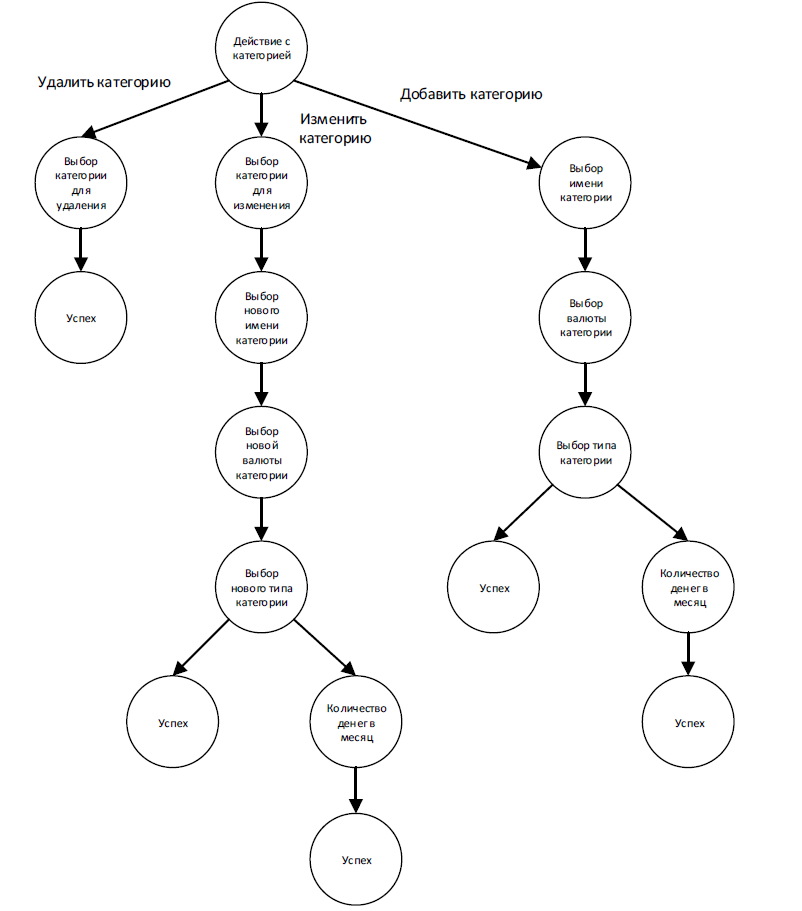
\includegraphics[scale=0.8]{category_service_scheme.png}
	\caption{Схема древовидной структуры вопросов по категориям}
	\label{fig:design:server:category_service_scheme}
\end{figure}

Пользователю на выбор даются 3 действия с категориями. При выборе удалить, предлагается список категорий для удаления. При выборе добавить, предлагается ввести имя категории, валюту, а также тип. Если тип категории – expense, то бот спустится ниже по дереву и задаст вопрос о том, сколько бы пользователь хотел тратить в месяц. Если категория – income, настройка категории будет считаться завершенной. При выборе изменить, предлагается список категорий для изменения. После выбора категории, запускается тот же сценарий, что и при добавлении.

Общая схема, описывающая процедуру обработки команд категорий, представлена на рисунке \ref{fig:design:server:categories_scheme}

\begin{sidewaysfigure}
\centering
	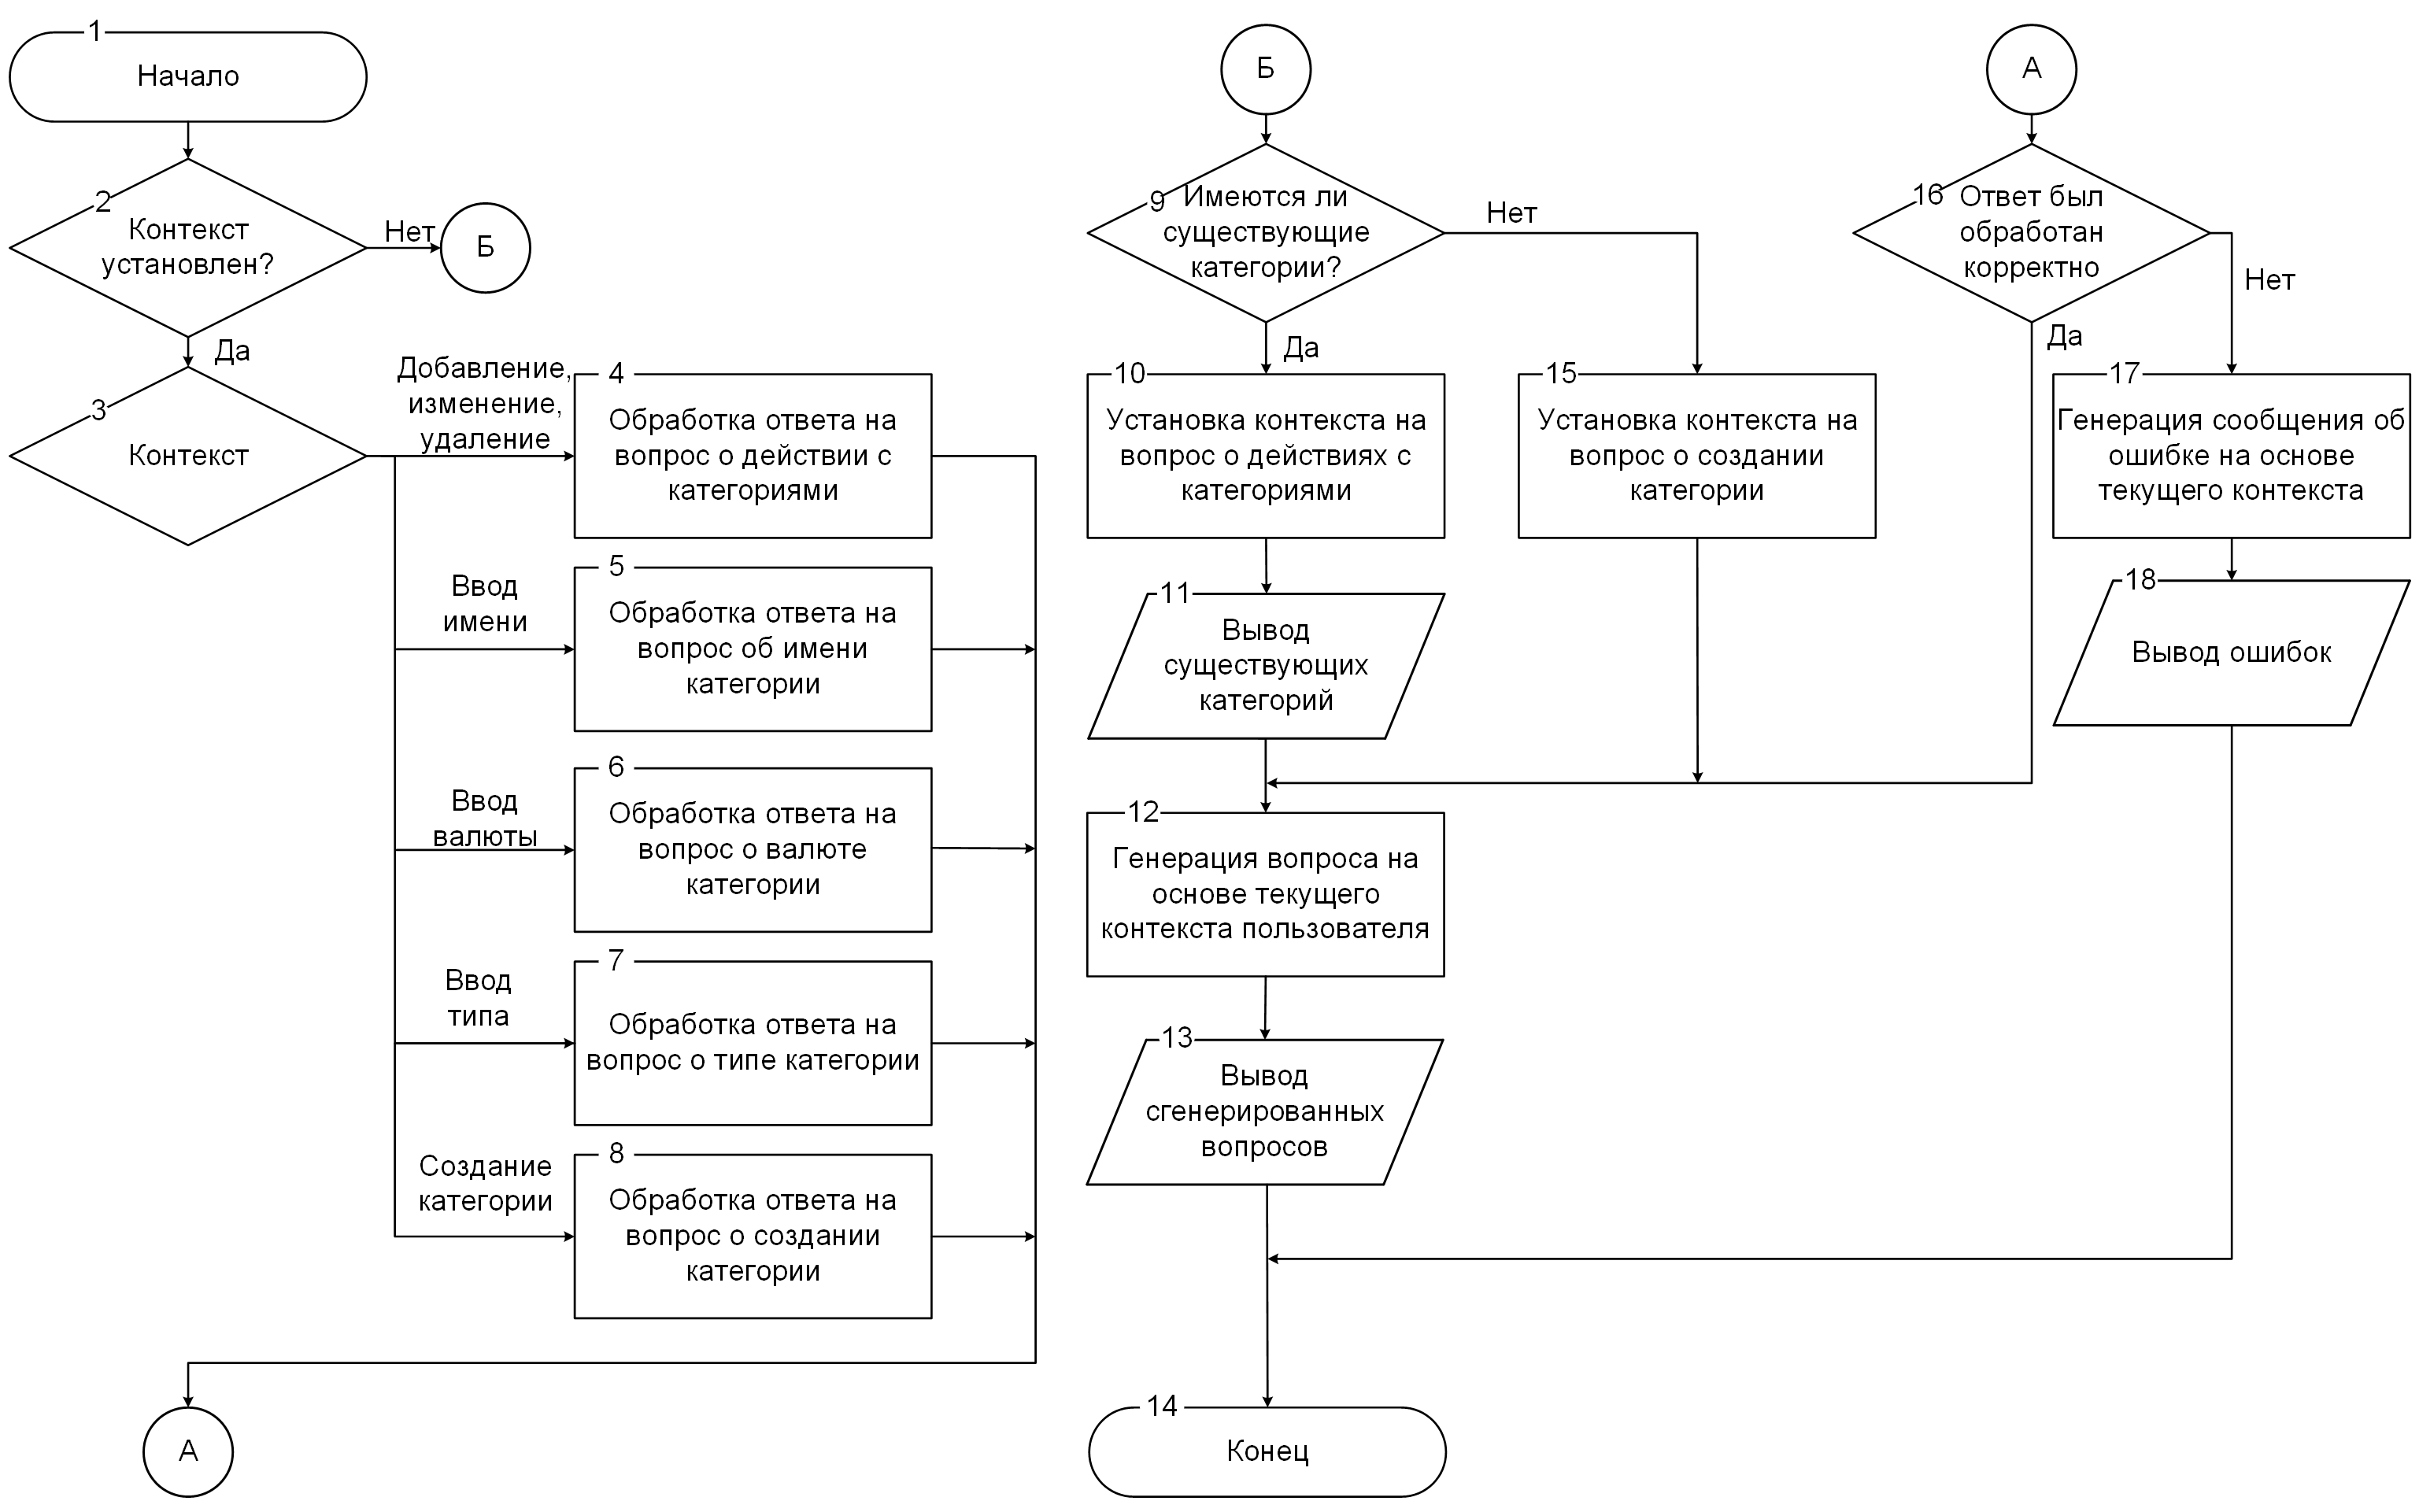
\includegraphics[scale=0.3]{categories_scheme.png}
	\caption{Общая схема работы сервиса категорий}
	\label{fig:design:server:categories_scheme}
\end{sidewaysfigure}

Главный метод класса – Handle}. Принимает на вход структуру Message. С помощью модуля работы с базой данных извлекает текущего пользователя и категории данного пользователя. В случае отсутствия категорий, добавляет в древовидную структуру узел с вопросом, желает ли пользователь добавить категории, и возвращает вопрос. Управление передается в генератор вопросов, который генерирует вопрос в соответствии с контекстом.

Метод HandleCategoryQuestion класса отвечает за обработку ответов
пользователей на вопросы бота. На вход принимает строку-ответ
пользователя, и структуру, описывающую самого пользователя.

С помощью структуры-словаря, по значению узла контекста
пользователя, управление передается в обработчик ответов.

\vskip 1.2in

\subsubsection{} OperationCommandHandlerService
\label{sec:design:server:OperationCommandHandlerService}

Обработчик команд /income и /expense. Реализует логику приложения,
отвечающую за операции. Содержит структуру типа Dictionary<string,
QuestionsHandlerDelegate>, которая представляет собой словарь, ключом
которого является название команды, значением – делегат, в который
передается управление.

Инициализация структуры выполняется методом \linebreak
InitializeQuestionsHandlerDictionary. Метод описан в листинге ниже:

\lstset{style=sharpc}
\begin{lstlisting}
private void InitializeQuestionsHandlerDictionary()
{
	_questionsHandlerDictionary = new Dictionary<QuestionsEnum, QuestionsHandlerDelegate>
	{
		{QuestionsEnum.OperationDate, ConfigureOperationDate },
		{QuestionsEnum.OperationSum, ConfigureOperationSum },
		{QuestionsEnum.OperationCategory, ConfigureOperationCategory}
	};
}
\end{lstlisting}

Метод устанавливает обработчики для ответов на вопросы о дате, сумме и выбранной категории. 

Как и класс CategoryCommandHandlerService, содержит структуру
\linebreak QuestionTree, представляющую собой дерево из вопросов для пользователя. На рисунке \ref{fig:design:server:operation_service_scheme} представлена схема данной структуры.

В начале выбирается категория для операции, далее запрашивается
сумма операции и дата. После введения всех данных, операция считается завершенной.

\begin{figure}[!h]
\centering
	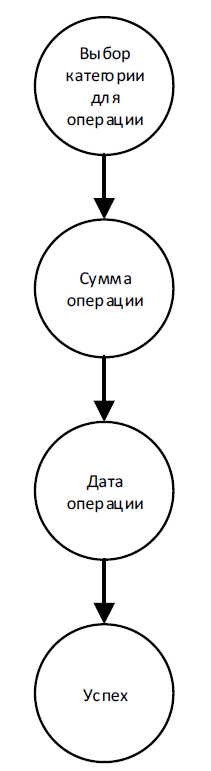
\includegraphics[scale=0.7]{operation_service_scheme.png}
	\caption{Схема структуры вопросов по категориям}
	\label{fig:design:server:operation_service_scheme}
\end{figure}

Главный метод класса – Handle. С помощью модуля работы с базой
данных извлекает текущего пользователя, а также в зависимости от команды /income или /expense устанавливает в контекст одно из значений перечисления CategoryTypeEnum, описанного в листинге ниже:

\lstset{style=sharpc}
\begin{lstlisting}
public enum CategoryTypeEnum
{
	Income,
	Expense
}
\end{lstlisting}

Далее управление передается в метод ConfigureOperationType, где с помощью модуля работы с базой данных извлекаются все категории
пользователя данного типа. Если таких категорий не найдено, с помощью сервиса генерации сообщений об ошибках ResultService,генерируется сообщение о том, что таких категорий не найдено. Если категории найдены, в базу данных записывается операция, а управление передается генератору вопросов.

Общая схема, описывающая процедуру обработки команд операций, представлена на рисунке \ref{fig:design:server:operations_scheme}

\begin{sidewaysfigure}
\centering
	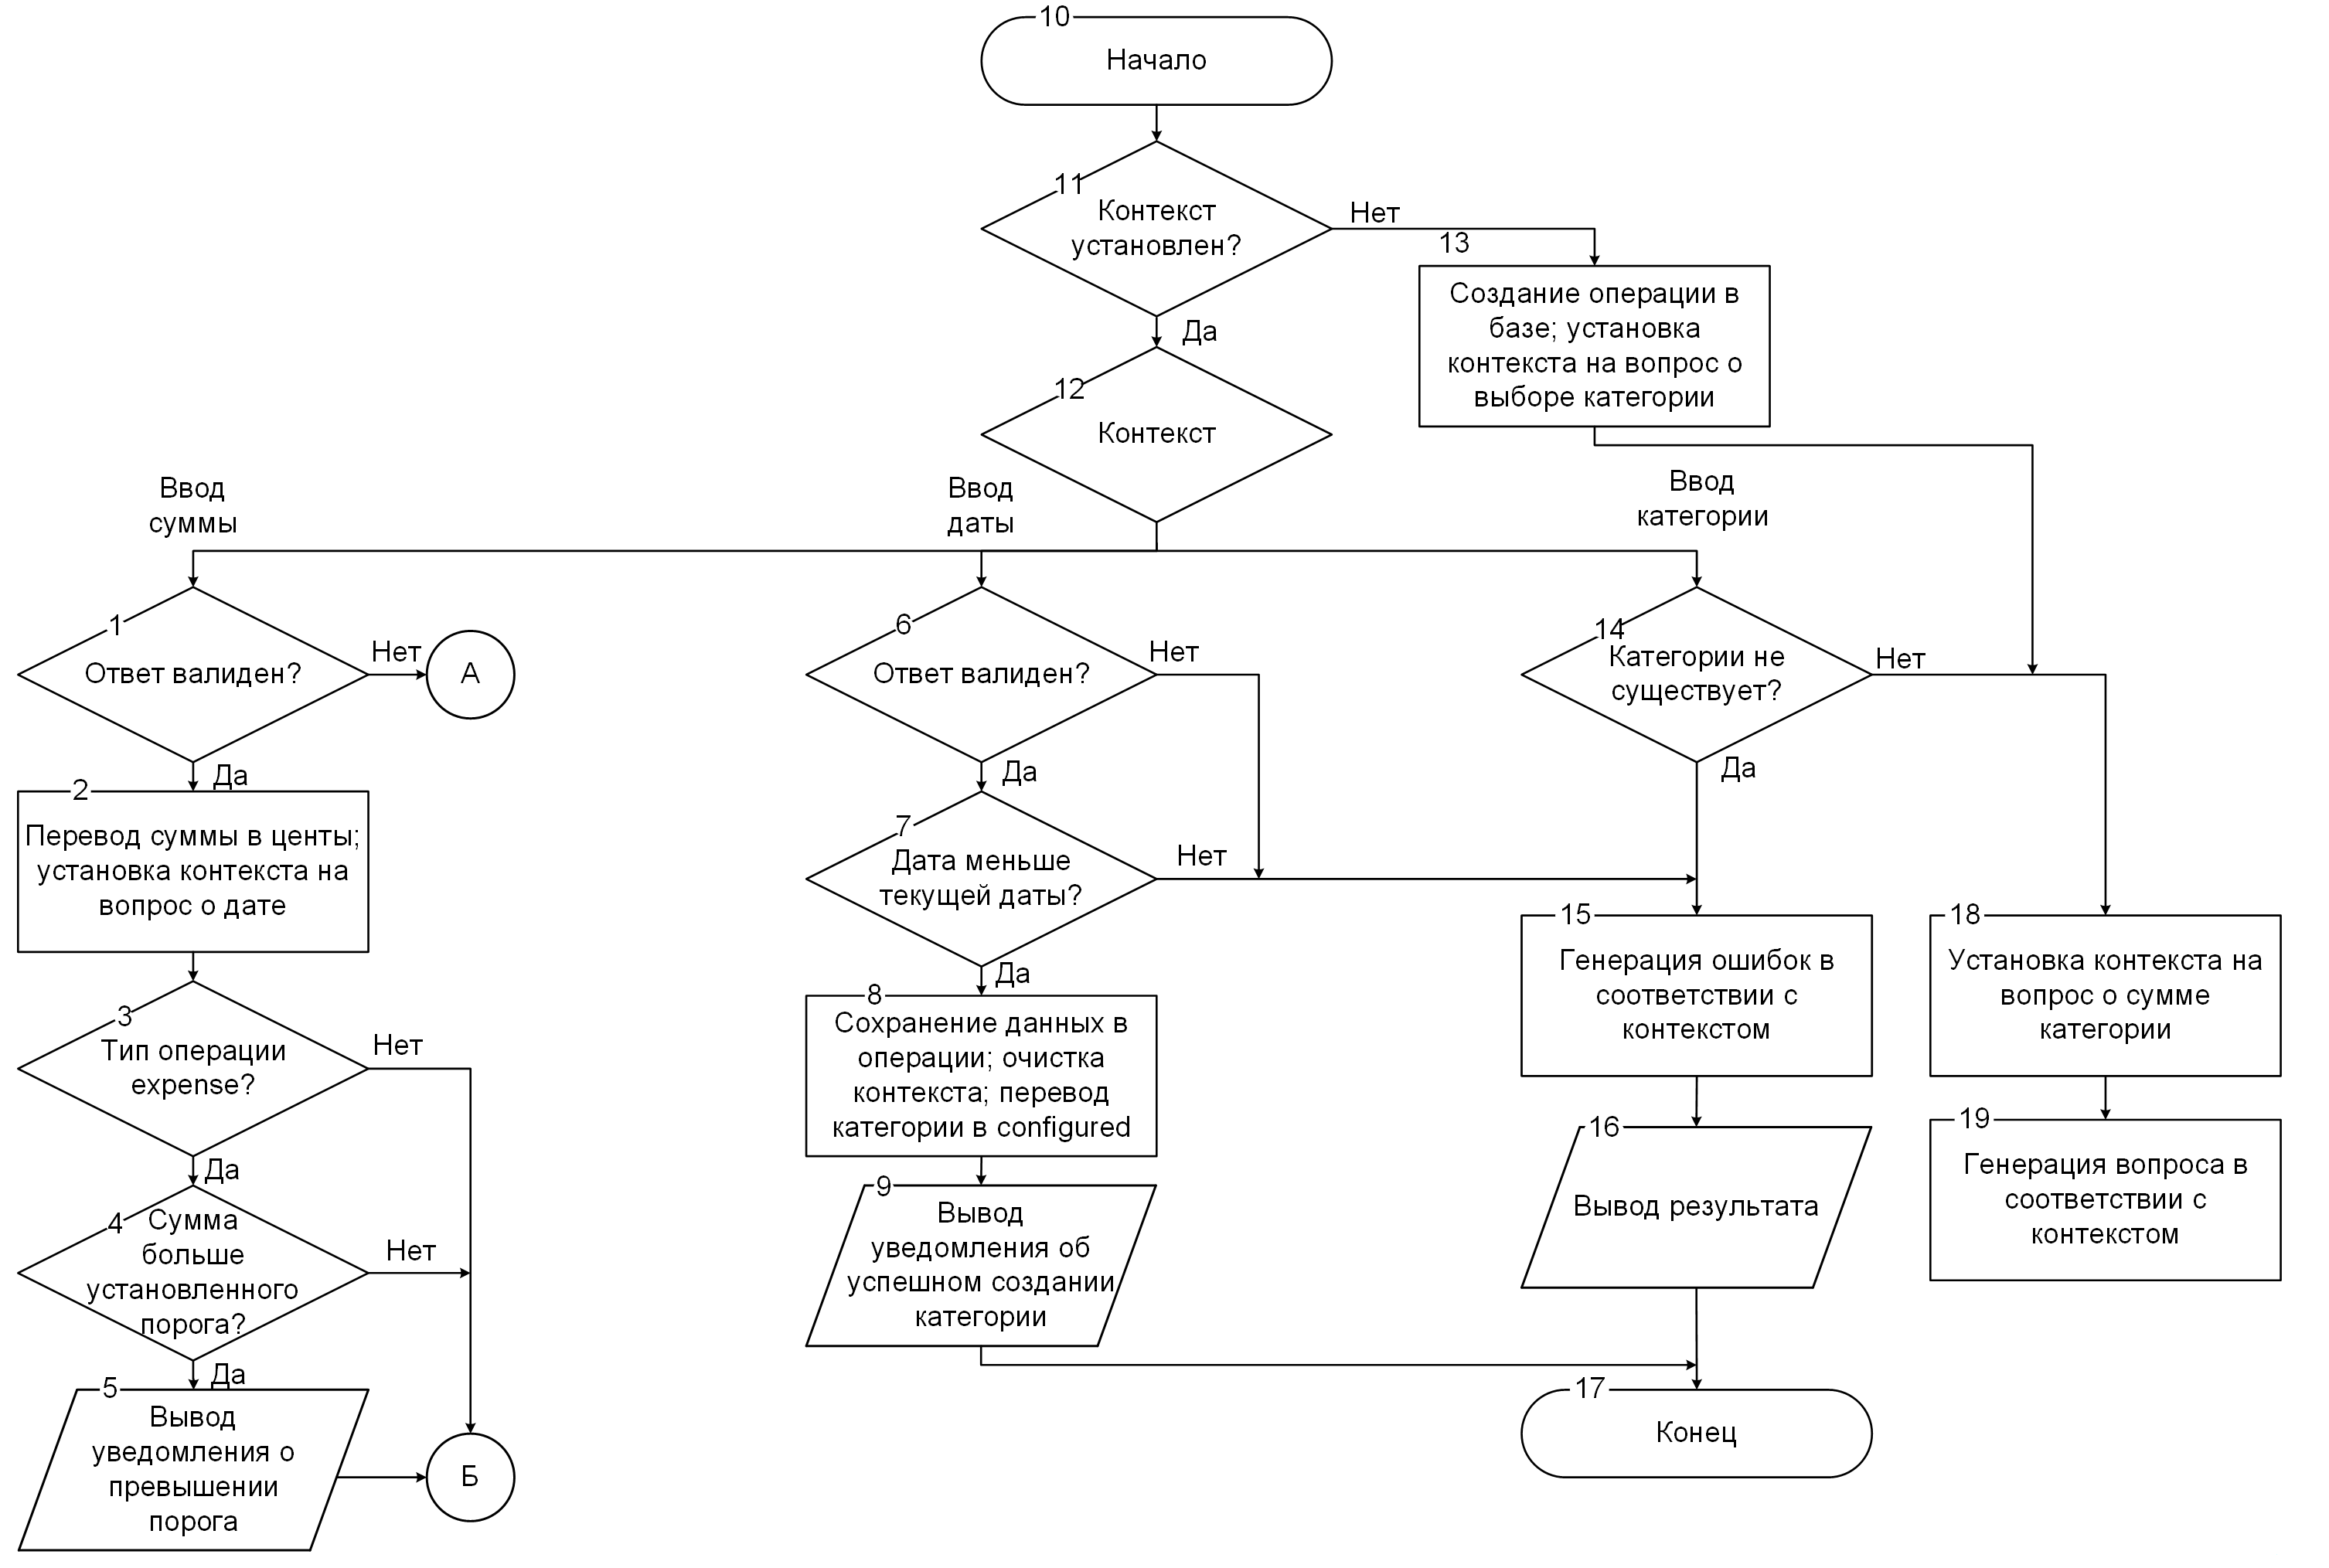
\includegraphics[scale=0.29]{operations_scheme.png}
	\caption{Общая схема работы сервиса категорий}
	\label{fig:design:server:operations_scheme}
\end{sidewaysfigure}


\newpage

Метод HandleOperationQuestion класса отвечает за обработку ответов пользователей на вопросы бота. На вход принимает строку-ответ пользователя, и структуру, описывающую самого пользователя.

\subsubsection{} UnhandledMessageService
\label{sec:design:server:UnhandledMessageService}

В случае, если бот не поддерживает данную команду, либо внутри программного средства было сгенерировано исключение, вызывается метод Handle класса UnhandledMessageService. В него передаются сведения о пользователе, сообщение пользователя, а также исключение. Обработчик упаковывает все данные в структуру UnhandledMessage и, с помощью модуля работы с базой данных, записывает её в базу. 

\newpage

Структура UnhandledMessage описана в листинге ниже:

\lstset{style=sharpc}
\begin{lstlisting}
public class UnhandledMessage : BaseModel
{
	public string Text { get; set; }

	public long ChatId { get; set; }

	public DateTime Created { get; set; }

	public Exception Exception { get; set; }
}
\end{lstlisting}

\subsubsection{} StatsCommandHandlerService
\label{sec:design:server:StatsCommandHandlerService}

Обработчик команды /stats. Реализует логику приложения, отвечающую за предоставление пользователю статистики по операциям. Содержит структуру типа Dictionary<string, QuestionsHandlerDelegate>, которая представляет собой словарь, ключом которого является название команды, значением – делегат, в который передается управление.

Инициализация структуры выполняется методом \linebreak InitializeQuestionsHandlerDictionary.

Как и в случае с классами CategoryCommandHandlerService и \linebreak OperationCommandHandlerService, данный класс имеет древовидную структуру, отвечающую за предоставление вопросов пользователю.

На рисунке \ref{fig:design:server:stats_service_scheme} представлена схема этой структуры для класса \linebreak StatsCommandHandlerService.

\begin{figure}[!h]
\centering
	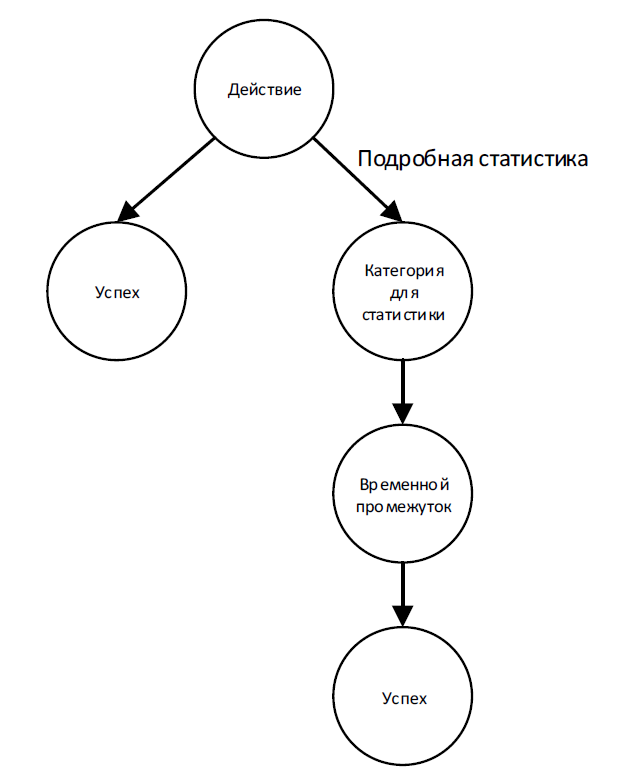
\includegraphics[scale=0.7]{stats_service_scheme.png}
	\caption{Схема древовидной структуры вопросов по статистике}
	\label{fig:design:server:stats_service_scheme}
\end{figure}

На выбор пользователю предлагаются 4 варианта: статистика по всем категориям, только income, только expense, либо подробная статистика. В случае выбора подробной статистики, бот запросит категорию для статистики, а также временной промежуток.

Для генерирования статистики используется сервис StatsService. В он себе содержит 2 перегрузки метода BuildStatistics. Первая используется для генерации подробной статистики, вторая – для
генерации статистики для группы категорий.

Основные методы модуля перечислены в таблице \ref{table:design:server:framework}.

\vskip 0.7in

\begin{longtable}{|>{\raggedright}p{0.3\textwidth}|
		 >{\raggedright}p{0.3\textwidth}|
		 >{\raggedright\arraybackslash}p{0.32\textwidth}|} 
	\caption{Классы и методы модуля обработки команд}
	\label{table:design:server:framework}\\

	\hline
	\centering Класс & \centering Метод & \centering\arraybackslash Описание \endfirsthead

	\caption*{Продолжение таблицы \ref{table:design:server:framework}}\\\hline
	\centering 1 & \centering 2 & \centering\arraybackslash 3 \\\hline \endhead

	\hline
	\centering 1 & \centering 2 & \centering\arraybackslash 3 \\
	\hline

	CommandService & ExecuteCommand(string command, Message message) & Извлекает из базы данных пользователя, исходя из контекста пользователя, передает управление в  \\

	& & классы-обработчики команд. В случае возникновения исключительной ситуации, вызывает обработчик UnhandledMessage \linebreak Service. \\ \hline

	CommandService & InitializeCommand
HandlerDictionary & Инициализирует словарь, ключом которого является команда, значением – делегат, в который передается управление. \\ \hline

	UnhandledMessage
Service & Handle(Message message, Exception exception) & Заполняет структуру UnhandledMessage данными из параметров и записывает её в базу. \\ \hline

CancelCommand
HandlerService & Handle(Message message) & Извлекает и базы данных текущего пользователя. Если он содержит ненулевой контекст, удаляет операцию, а также категорию из базы данных. Выставляет контекст пользователя в null. Сохраняет пользователя в базу. \\ \hline

HelpCommand
HandlerService & Handle(Message message) & Возвращает сообщение со списком команд, поддерживаемых ботом. \\

StartCommand
HandlerService & Handle(Message message) & Извлекает текущего пользователя из базы данных. Если пользователя с данным ChatId не существует, создает нового пользователя, а также 2 стандартных категории. Сохраняет пользователя в базу данных. \\ \hline

CategoryCommand
HandlerService & Handle(Message message) & Извлекает пользователя, а также его категории из базы данных. В случае, если категорий не существует, добавляет в древовидную структуру еще один узел и передает управление сервису построения вопросов. Если категории существуют, передает управление в сервис построения вопросов. \\ \hline

CategoryCommand
HandlerService & HandleCategoryQuestion
(string answer, User user) & Отвечает за обработку ответов пользователя на вопросы бота. Извлекает из контекста пользователя текущий узел и использует его как ключ для поиска метода, отвечающего за обработку, в словаре. Передает управление в метод-обработчик.
 \\

& & 
В случае, если в словаре не найден данный ключ, возвращает сообщение об ошибке. \\ \hline

CategoryCommand
HandlerService & InitializeQuestionTree() & Инициализирует древовидную структуру, использующуюся для реализации контекста. \\ \hline

CategoryCommand
HandlerService & InitializeQuestions
HandlerDictionaty & Инициализирует словарь, использующийся для обработки ответов пользователя. \\ \hline

CategoryCommand
HandlerService & ConfigureCategory
Action(string answer, User user) & Обрабатывает ответ пользователя на вопрос о действии с категориями. В случае, если ответ пустой, либо не содержит одного из нужных ответов, возвращается сообщение об ошибке.
В зависимости от ответа пользователя, проводятся соответствующие операции, а в контекст пользователя устанавливается узел-сын текущего узла. Управление передается в генератор вопросов. \\

Operation
Command
HandlerService & Handle(Message message) & Обрабатывает команды /income и /expense. Извлекает из базы данных текущего пользователя, устанавливает в контекст пользователя начальный узел структуры контекста. Управление передается в метод ConfigureOperationType. \\ \hline

Operation
Command
HandlerService & ConfigureOperationType
(CategoryTypeEnum type, User user) & Отвечает за обработку запроса пользователя. Если категорий с данным типом не существует, возвращается сообщение об ошибке.
В контекст устанавливается узел-сын текущего узла.
Управление передается в генератор вопросов. \\ \hline

Operation
Command
HandlerService & HandleOperation
Question
(string answer, User user) & Отвечает за обработку ответов пользователя. Используя контекст пользователя, передает управление в методы-обработчики.
В случае, если в словаре не найдено такого ключа, возвращается сообщение об ошибке. \\ 

StatsCommand
HandlerService & Handle(Message message) & Обрабатывает команду /stats. Извлекает из базы данных текущего пользователя, а также его категории. Если категорий не существует, возвращается сообщение об ошибке.
В контексте пользователя устанавливается узел контекста. Управление передается в генератор вопросов. \\ \hline

StatsCommand
HandlerService & HandleStatsQuestion
(string answer, User user) & Отвечает за обработку ответов пользователя на вопросы о статистике. С помощью контекста пользователя, управление передается в методы-обработчики. Если в словаре не найден такой ключ, возвращается сообщение об ошибке. \\ \hline

StatsCommand
HandlerService & ConfigureStatsAction
(string answer, User user) & Отвечает за обработку ответа пользователя на вопрос о действии со статистикой. Если ответ пустой, либо   \\ 

& & не содержит подходящего варианта, возвращается сообщение об ошибке. В зависимости от ответа пользователя, управление передается в сервис-генератор статистики. Если пользователь выбрал подробную статистику для одной категории, узел контекста принимает значение узла-сына, управление передается в генератор вопросов. \\ \hline

StatsCommand
HandlerService & ConfigureStatsCategory
(string answer, User user) & Отвечает за обработку ответа пользователя на вопрос о категории для статистики. Если ответ пустой, возвращается сообщение об ошибке. Если категория с таким именем у пользователя отсутствует, возвращается сообщение об ошибке. В контекст пользователя устанавливается категория, узел контекста принимает значение узла-сына. Управление передается в генератор вопросов.\\ \hline

\end{longtable}

\subsubsection{} Модуль работы с базой данных
\label{sec:design:server:db}

Основная задача данного модуля состоит в принятии запросов от модуля
обработки команд для построения нужных моделей данных. Может быть
размещен на отдельном сервере для увеличения производительности и снятия нагрузки с основных серверов.

В приложении используются следующие модели данных:

\begin{itemize}
	\item Category – модель данных категории;
	\item Operation – модель данных операции;
	\item User – модель данных пользователя;
	\item UnhandledMessage – модель данных сообщения об ошибке;
	\item Chat – модель данных чата;
	\item Logs – модель данных логирования приложения;
	\item LogRequest – модель данных логирования запроса;
	\item LogResponse – модель данных логирования ответа;
	\item UserStatus – модель данных статуса пользователя;
	\item Context – модель данных контекста пользователя.
\end{itemize}

Данный модуль был спроектирован с соблюдением паттерна «репозиторий», который делает структуру данного модуль гибкой к изменениям. Если понадобится замена использующейся в проекте в данное время базы данных MongoDB, это можно будет сделать легко, заменив лишь класс с обращениями к драйверу базы данных.

Так как, на данный момент, в проекте используется MongoDB, то главным классом в модуль работы с базой данных является MongoService.

В нем происходит настройка и конфигурирование доступа к драйверу базы данных, а также предоставляется доступ к коллекциям.

Для каждой модели данных есть свой репозиторий:

\begin{itemize}
	\item CategoryDocumentService;
	\item OperationDocumentService;
	\item UnhandledMessageDocumentService;
	\item UserDocumentService;
	\item ChatDocumentService;
	\item LogsDocumentService;
	\item UserStatusesDocumentService.
\end{itemize}

Все сервисы реализуют интерфейс IDocumentService<T>, описывающий базовые методы, которые должны быть реализованы каждым из сервисов. Структура интерфейса описана в листинге ниже:

\lstset{style=sharpc}
\begin{lstlisting}
public interface IDocumentService<T>
{
	Task InsertAsync(T item);

	Task UpdateAsync(T item);

	Task DeleteAsync(string id);

	Task<T> GetByIdAsync(string id);

	string GenerateNewId();
}
\end{lstlisting}

Также, все сервисы реализуют абстрактный класс \linebreak BaseDocumentService, в котором реализованы все базовые методы, нужные для работы приложения.

Описание методов класса BaseDocumentService находится в таблице \ref{table:design:server:db}.

\begin{longtable}{|
		 >{\raggedright}p{0.42\textwidth}|
		 >{\raggedright\arraybackslash}p{0.53\textwidth}|} 
	\caption{Методы класса BaseDocumentService}
	\label{table:design:server:db}\\

	\hline
	\centering Метод & \centering\arraybackslash Описание \endfirsthead \hline

	GenerateNewId() & Генерирует новый идентификатор. \\ \hline
	
	InsertAsync(T document) & Асинхронно вставляет элемент в коллекцию. \\ \hline

	UpdateAsync(T document) & Асинхронно обновляет элемент в коллекции. \\ \hline

	DeleteAsync(string id) & Асинхронно удаляет элемент из коллекции. \\ \hline

	GetByIdAsync(string id) & Асинхронно производит поиск и возвращает элемент из коллекции. \\ \hline

\end{longtable}